% KERdoc.tex V1.0, 14 June 2004

\documentclass{KERauth}
\usepackage{listings}
\usepackage{color}
\usepackage{amssymb}
\usepackage{pifont}% http://ctan.org/pkg/pifont
\newcommand{\cmark}{\ding{51}}%
\newcommand{\xmark}{\ding{55}}%

\setcounter{tocdepth}{3}
\usepackage{graphicx}
\usepackage{oz}
\usepackage{float}
\usepackage{booktabs}
\usepackage{verbatim}
\usepackage{moreverb}
\usepackage{setspace}

\begin{document}
\KER{1}{24}{00}{0}{2004}{S000000000000000}

%\runningheads{}{A demonstration of The Knowledge Engineering Review class file}

%\doublespacing
\onehalfspacing

\title{A Blockchain Based Decentralised Booking System}

\author{Naipeng Dong$^1$, Guangdong Bai$^2$, Lung-Chen Huang$^3$, Edmund Kok Heng Lim$^4$ and Jin Song Dong$^{5}$}
\address{$^{1,3,4,5}$School of Computing, National University of Singapore, COM$1$, $13$ Computing Drive, $117417$, Singapore\\ ~$^{2,5}$School of Information and Communication Technology, Griffith University, N$44$ $2.28$, $170$ Kessels Road Nathan, QLD, $4111$, Australia\\
\email{$^1$dcsdn@nus.edu.sg}, $^2$g.bai@griffith.edu.au, $^3$lungchenhuang@u.nus.edu, $^4$e0335737@u.nus.edu, $^5$dcsdjs@nus.edu.sg}


\begin{abstract}
Blockchain technology has rapidly emerged as a decentralised trusted network to replace the traditional centralised intermediator. Especially, the smart contracts that are based on blockchain allow users to define the agreed behaviour among them, the execution of which will be enforced by the smart contract. Based on this, we propose a decentralised booking system that uses the blockchain as the intermediator between hoteliers and travellers. The system enjoys the trustworthiness of blockchain, improves efficiency and reduces the cost of the transitional travel agencies. The design of the system has been formally modelled using the CSP\# formal language and has been formally verified using the model checker PAT. We have implemented a prototype decentralised booking system based on the Eethereum ecosystem.
\end{abstract}

\section{Introduction}

The blockchain technology has rapidly emerged in recent years (Nakamoto (2019), Buterin (2019), Swan (2015)), especially when the concept of smart contract
was first introduced to and later relied on the technology (Morris (2019), Cachin (2019), Schwartz \emph{et al.} (2014)). Once the smart contract code is deployed to the
blockchain, it can be executed by any computer node that keeps the same historical record of transactions as
other nodes. This makes it difficult to be compromised with a single node on the network, unlike centralized
platforms that could be easily breached and prone to the failure of single point. However, decentralized
platforms are still in its infancy. Although some communities and companies have proposed some use cases
for the logistics (DHL (2019), Marr (2019)) and insurance industry (CBInsights (2019), Sarasola (2019)), its use cases are lacking in different domains. To give a more concrete
example of using the smart contract, we design a fundamental architecture of a decentralized hotel booking
system.

Most travelers would have hard times finding a hotel room for their next journey. They would possibly
browse through pages of entries on online travel agencies such as \emph{Booking.com} or \emph{Agoda.com}. As
we can imagine, it is time-consuming that each time a search result appears on the screen, they have to
delve into the deals one by one, which could be overlapping in the last search results. In order to alleviate
this monotonous experience, we shall leverage the blockchain technology and allow our search requests to
be deployed as smart contracts such that the process of discovery is left to the decentralized system, where
hoteliers can easily match their rooms with the criteria required by a traveler.

Our approach is to provide users with an interface where they can draft their booking request with the
requirement of a hotel room in a domain-specific language, which is similar to a real contract in a human-readable form. Thereafter, the interface compiles the request into a machine-readable form and injects some
predefined functions. Later, the user can deploy the request onto the blockchain. Once the request is visible
to other nodes, hoteliers can propose offers by invoking a function in the request. When the user is notified
of new proposals, the interface automatically starts a selection process of the proposals depending on the
request criteria from the user, showing the matched results. At the end, the user and one of the hoteliers seal
a deal.

To ensure the correctness of the design, we model the system using the CSP\# (Communicating Sequential Programs sharp) formal language (Sun {\it et al.} (1999)), as CSP\# integrates the high-level modeling operators of CSP with low-level procedural codes in C\# language and supports custom data structures which is extensively used in our model to represent the behaviors of the blocks and the blockchain. We verify the design using the model checker PAT (Process Analysis Toolkit, available at pat.comp.nus.edu.sg) which supports the CSP\# models as input. The formal model is comprehensive, containing not only the behaviour of the smart contract, the hoteliers and the travellers, but also contains the blockchain mechanism.

In addition, we have implemented a prototype booking system based on the Ethereum ecosystem (Ethereum (2019)), and tested the prototype system on a Ethereum Virtual Machine (EVM). The booking system contains three components: the hotelier, the traveler and the smart contract. The EVM mainly contains the EVM nodes, the miner nodes. We use \emph{Truffle} to compiler the smart code and deploy the compiled bytecode to the EVM nodes. In addition, we installed a web server to test the hotelier and traveller websites.

\section{Background}

In this work,
we use the CSP\# as the language to formally model the design.
This language is supported by the automatic model checker PAT. Thus, we use PAT to automatically verify a set of desired properties of our design. The syntax of this language and the model checker PAT are briefly introduced in the first section. After verifying the correctness of the design, we implemented the design based on EVM, which is described in the second part.

\subsection{CSP\# and PAT}

The CSP\# is a rich modelling language that contains both high level modelling operators in the traditional CSP language and programmer-favored low-level constructs like variables, arrays, if-then-else, while, etc..  It offers great flexibility to model systems with complicated structures, like blockchain. A system is modelled as a process in CSP\#. And the operators in CSP\# is defined as follows.

\begin{displaymath}
\hspace{1.5cm} \text{Process } P, Q ::= \\
\hspace{3.2cm}Stop \hspace{1.8cm} - \text{deadlock} \\
\hspace{3cm} | Skip \hspace{2cm} \ \ \ - \text{termination} \\
\hspace{3cm} | [b]P \hspace{2cm} \ \ \ - \text{state guard} \\
\hspace{3cm} | e \rightarrow  P \hspace{2cm} - \text{event prefixing} \\
\hspace{3cm} | e \{program\} \rightarrow P \ \ \ - \text{data operation prefixing} \\
\hspace{3cm} | c?d \rightarrow P(d) \hspace{1cm} \ - \text{channel input} \\
\hspace{3cm} | c!d \rightarrow P \hspace{1.5cm} \ - \text{channel output} \\
\hspace{3cm} | P; Q \hspace{2cm} \ - \text{sequence} \\
\hspace{3cm} | P \sqcap Q \hspace{2cm} - \text {internal choice} \\
\hspace{3cm} | P \square Q \hspace{2cm} \ - \text {external choice} \\
\hspace{3cm} | if\ b\ then\ P\ else\ Q \ - \text {conditional branch} \\
\hspace{3cm} | P || Q \hspace{2cm} - \text{synchronous} \\
\hspace{3cm} | P ||| Q \hspace{1.9cm} - \text{asynchronous}
\end{displaymath}
%
where $P$ and $Q$ are $processes$, $b$ is a condition, $e$ is a simple event, $program$ is a block of code that is atomically executed and $c$ is a synchronized communication channel.

The deadlock process is $Stop$, meaning the process does absolutely nothing. Process $Skip$ means the process termites immediately. Process $[b]P$ is a guarded process - the process behaves as $P$ if $b$ is satisfied. Process $e \rightarrow  P$ is event prefixing - the process performs event $e$ (a simple event is a name for representing a observation) and then behaves as $P$. Process $e \{program\} \rightarrow P$ is similar to event prefixing. The difference is that the $\{program\}$ attached with event $e$ allows us to write assignments which update global variables. Process $c?d \rightarrow P(d)$ is channel input - the process reads a value $d$ from channel $c$, thus $d$ is known in the subsequent process $P$. Process $c!d \rightarrow P$ is channel output - the process outputs value $d$ in channel $c$. Process $P; Q$ concatenates two processes $P$ and $Q$ sequentially. Process $P \sqcap Q$ is internal choice - the process either chooses $P$ or $Q$ to execute. If $P$ performs an event first, then $P$ takes control; Otherwise $Q$ takes control. $P \square Q$ is external choice. Differing from the internal choice, the external choice is resolved by the environment. Process $if\ b\ then\ P\ else\ Q$ is straight forward: if $b$ is true, the process behaves as $p$; Otherwise behaves as $Q$. Both $P || Q $ and $P ||| Q$ model parallel processes $P$ and $Q$. The difference is that the form one requires $P$ and $Q$ to synchronise on the shared events whereas in the later process, $P$ and $Q$ interleave.

PAT is a self-contained framework which supports simulating and reasoning and verifying concurrent systems. It has user friendly interfaces, featured model editor and animated simulator. Most importantly, PAT implements various model checking techniques catering for different properties such as deadlock-freeness, reachability and LTL properties that are useful for our system verification. To achieve good performance, advanced optimization techniques are implemented in PAT, e.g. partial order reduction, symmetry reduction, process counter abstraction, parallel model checking. So far, PAT has 4370+ registered users from 1341+ organizations in 150 countries and regions.

\subsection{Ethereum}

The Ethereum ecosystem serves as a runtime environment for smart contracts. It provides a language \emph{Solidity} to write smart contracts. The smart contracts need \emph{Gas} to be executed. And gas can only be bought using the cryptocucrency \emph{Ether} Provided by Ethereum. It mainly involves the following parts (Ethereum (2019), Modi (2019), Buterin (2019)):

\begin{itemize}
    \item EVM nodes: The EVM runs smart contract bytecode. Each node runs an instance of the EVM. Once written, the contracts have to be deployed on the EVM. Users can interact with the contracts that are on the EVM. The EVM node is a host for the Ethereum network. There can be many EVM nodes serving one network, in that sense the Ethereum network is decentralised.
    \item Mining nodes: The mining nodes (a.k.a. miners) form the basic blockchain. Each block contains data and smart contract code, and holds a copy of the blockchain. The mining nodes are required to verify and add blocks to the chain and in the process get paid in Ether. Every transaction requires Gas to run. Gas is the measure of the amount of Ether that is required to run.
    \item Externally owned account: It represents a user. When a new account is created, a private public key pair is created. The Externally owned account is the public key of the account.
    \item Wallet: It is a software that is associated to user accounts. One user may have more than one account in one wallet. The wallet is an important component as it is the software that tracks the amount of Ether one has. Mining nodes also require a wallet to store the ether earned. Most wallets will show transactions made; these transactions are identified by their hash values.
    \item Smart contracts: Smart contracts are programs that exist on the EVM. They can accept inputs and based on the inputs, can produce an action whether it is to read a value from the blockchain or to write a value to the blockchain. Smart contracts are the key to interacting with the blockchain programmically.
    \item Uer interface: It refers to any interface that is interacting with a smart contract on the EVM. User interfaces together with smart contracts are known as DApps or decentralised apps.
\end{itemize}


\section{System design}

To more clearly illustrate the workings of our system, the system sequence diagram in Figure~\ref{fig:overview} describes
how travelers and hoteliers interact on the decentralized booking platform.

\begin{figure}[t]
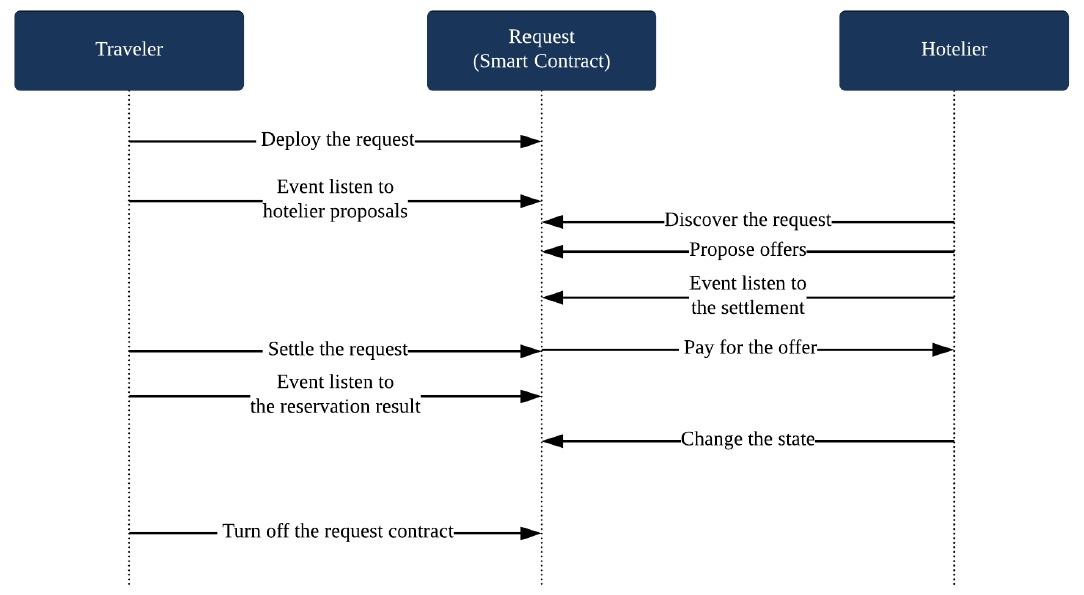
\includegraphics[width=\textwidth]{mec.jpg}
\caption{Overview of the system design}
\label{fig:overview}
\end{figure}

Once the smart contract is deployed on the EVM, a traveler can put a request to the smart contract and then listens to the contract for any response. A Hotelier listens to the contract and once discovers a request he proposes his offer. After that the hotelier listens to the contract for response. When the traveler accepts the offer, he settles the request and then pay the deposit. On receiving the deposit payment, the hotelier change the room into unavailable and informs the smart contract. Finally, the traveler disable the request.

In more details, our system contains three roles \emph{user}, \emph{miner}, and the {smart contract}.
\begin{itemize}
    \item A user could be a traveler or hotelier who sends a transaction by invoking a function that includes
the address of the user, function name, gas, and gas price. A traveler can invoke Fetch to acquire the latest
set of proposals submitted by hoteliers, or to Settle for a specific proposal.
A hotelier can invoke Propose
to send their proposals to the request.
\item Miners form the basic blockchain network. Each miner has its own transaction pool $TxPool$ that continuously receives a new transaction with
gas greater than zero. Moreover, $TxBlock$ to be executed by a miner also finds the new transactions with
more than or equal to a specified transaction $gasPrice$ from the pool.
\item The smart contract is named as the Request. The request deployed on the blockchain is a smart contract that accepts proposals
and can be invoked by the users.
\end{itemize}


\section{System modelling}

First of all, we define a list of constants that are used in the model. Then we divid the model into two parts: the \emph{user} behavour in Section~\ref{sec:user} and the \emph{Miner} behaviour in Section~\ref{sec:miner}. The miner part includes the behaviour of the EVM nodes, the Mining nodes, and the smart contract. Since these behaviours are closely related, we do not separate them.
\begin{center}
\begin{boxedverbatim}
enum {off, on, switchOp, proposeOp, fetchOp, settleOp, proposedFrom,
      Function, ProposeFunction, settled, na, proposed, SwitchFunction,
      FetchFunction, SettleFunction, newcomer};
\end{boxedverbatim}
\end{center}

\subsection{user}\label{sec:user}
A user has an address $addr$. The user would like to execute $function$ and would like to pay a fund $val$ plus some gas amount $gas$ with price $gasPrice$. To do so, the user broadcasts the transaction to all miners. The reason that the user needs to specify the gas amount and gas price is that the gas price is changing according to the demand and supply; to be clear on how much the user pays the miner for executing the function, the user specifies the current gas price and the amount of gas the user would like to pay.
For simplicity, we assume the user sends the transactions to miners in order, as this will not affect the results we would like to check. The process of sending a transaction to miner $i$ is modelled as $TxBrdcst(i, addr, val, gas, gasPrice, function)$. When the miner index $i$ is correct (i.e., $i$ is smaller than the maximum number of miners), this process sends a transaction to the $i$-th miner with the parameters $addr, val, gas, gasPrice, function$, and then continues to sends the transaction to the next miner. If the miner index reaches the top, meaning that the user has sends to every miner, then the process terminates with $Skip$.

\begin{center}
\begin{boxedverbatim}
User(addr, val, gas, gasPrice, function) =
            TxBrdcst(0, addr, val, gas, gasPrice, function);

TxBrdcst(iter, addr, val, gas, gasPrice, function) =
  atomic{
    if (iter < M) {
      mnet[iter]!addr.val.gas.gasPrice.function ->
      TxBrdcst(iter+1, addr, val, gas, gasPrice, function) }
    else {
      Skip } };
\end{boxedverbatim}
\end{center}

\subsection{Miner}\label{sec:miner}

The miner has two processes running in parallel: process $TxPool(i)$ which receives transactions and puts them into a pool, and process $TxInsert$ which includes the transactions in the pool into a block and initiates the mining.

The miner $i$ receives the transactions in the process $TxPool(i)$. On receiving a transaction with parameters, the miner first checks whether the sender i.e., the user with address $addr$ has enough funds and gas, if so, the miner inserts the transaction into his transaction pool $TxInsert(i, addr, val, gas, gasPrice, function)$, otherwise, the miner keeps waiting for another transaction, i.e., returning back to process $TxPool(i)$.

\begin{center}
\begin{boxedverbatim}
TxPool(i) =
  mnet[i]?addr.val.gas.gasPrice.function ->
  if (userWallet[i][addr] >= (val + (gas * gasPrice)) && gas > 0)
        {TxInsert(i, addr, val, gas, gasPrice, function) }
  else {TxPool(i) };
\end{boxedverbatim}
\end{center}

When inserting a transaction into a pool of miner $i$, the miner first check whether the pool is full, i.e., the current transactions in $i$ ($PoolPtr[i]$ is smaller than the max $poolSize$). If not, the miner receives the transaction in the pool by updating the address, the value, the gas, the gasPrice and the function to the pool of miner $i$. At the end, we update the pointer of the transaction pool to the next empty position. After
updating the transaction pool, the miner sends a single of $newcommer$ to the channel $datach$ for miner $i$ to initiate the block forming. Finally the process goes back to $TxPool(i)$ to listen to a new transaction. Note that before updating the transaction pool, we double check whether the current empty pool position is really empty by checking whether the gas for the current position is $0$. If the current position is not empty, the process move to the next position and tries to insert the transaction to the pool. If the transaction pool is full, the transaction pointer is reset to $0$ and then the transaction is inserted into the transaction pool, meaning to form transactions for the next block. We notice that if there are more than the maximum amount of transactions received in the pool before a block is formed, the pool will be reset to new ones. In our model, the total transactions are less than the maximum transitions in a pool, so this will not happen.

\begin{center}
\begin{boxedverbatim}
TxInsert(i, addr, val, gas, gasPrice, function) =
  if (poolPtr[i] < poolSize) {
    if (poolTxGas[i][poolPtr[i]] == 0) {
      txReceive{
        var ptr = poolPtr[i];
        poolTxAddr[i][ptr] = addr;
        poolTxVal[i][ptr] = val;
        poolTxGas[i][ptr] = gas;
        poolTxGasPrice[i][ptr] = gasPrice;
        poolTxFunction[i][ptr] = function;
        poolPtr[i]++;} ->
      datach[i]!newcomer ->
      TxPool(i) }
    else {
      next{poolPtr[i]++;} ->
      TxInsert(i, addr, val, gas, gasPrice, function) } }
  else {
    next{poolPtr[i] = 0;} ->
    TxInsert(i, addr, val, gas, gasPrice, function)};
\end{boxedverbatim}
\end{center}

The process $TxBlock(i)$ include available transitions into a block. When the number of transactions in the pool is smaller than the pool size and the channel for receiving transactions is not empty, the process receives a signal that a new transaction has been inserted into the transaction pool. Otherwise the process sets the pointer $inPoolPtr(i)$ to $0$ and goes back to the process $TxBlock(i)$.

On receiving the signal, the miner checks whether the gas for this transaction is $0$ indicating there is no transaction in the pool.
%
\begin{itemize}
\item If there is no transaction in the pool and the block size is bigger than $1$, meaning all the transactions have been included  the block, the miner starts mining  block by in the calling $Miner(i, 0)$. If there is no transaction in the pool and the block size is smaller than $1$, meaning there is no transaction in the block, then the process goes back to $TxBlock(i)$.

\item If there are transactions in the pool, the miner checks whether the total gas for the current block reaches the top limit and checks whether the current transaction in the pool provides enough gas to execute the function. If so, the miner include the transaction in the block, by copying the address, value, gas, gas price and function into the block. In addition, the miner update the total gas of the block and set the position of the transaction in the pool to be $0$ indicating that the transaction in the pool has been included into the block. Furthermore, the pointer in the pool will move to the next and the size of the block increase by $1$. After updating the current transaction in to pool, the process goes back to $TxBlock(i)$ to include the next transaction into the pool, until all transactions have been included, i.e., the pointer $inPoolPtr[i]$ is bigger than the $poolSize$. If the current transaction in the pool fails to provide enough gas, the miner simply ignores the transaction and moves to the next one. If the total gas has reached the top limit and there is transaction in the block, the miner starts mining. If the total gas reaches the top, but somehow there is no transaction in the block, the process goes back.
\end{itemize}

\begin{center}
\begin{boxedverbatim}
TxBlock(i) =
  if (inPoolPtr[i] < poolSize) {
    if (!call(cempty, datach[i])) {
      datach[i]?newcomer ->
      if (poolTxGas[i][inPoolPtr[i]] == 0) {
        if (blkSize[i] >= 1) {
          Miner(i, 0)}
        else { TxBlock(i) }	}
      else {
        if (blkTotalGas[i] + poolTxGas[i][inPoolPtr[i]] <= blkGasLimit) {
          if (poolTxGasPrice[i][inPoolPtr[i]] >= gasPriceCondition) {
            txInclude{
              var pIter = inPoolPtr[i];
              var bIter = blkSize[i];
              blkTxAddr[i][bIter] = poolTxAddr[i][pIter];
              blkTxVal[i][bIter] = poolTxVal[i][pIter];
              blkTxGas[i][bIter] = poolTxGas[i][pIter];
              blkTxGasPrice[i][bIter] = poolTxGasPrice[i][pIter];
              blkTxFunction[i][bIter] = poolTxFunction[i][pIter];
              blkTotalGas[i] = blkTotalGas[i] + poolTxGas[i][pIter];
              poolTxAddr[i][pIter] = 0;
              poolTxVal[i][pIter] = 0;
              poolTxGas[i][pIter] = 0;
              poolTxGasPrice[i][pIter] = 0;
              poolTxFunction[i][pIter] = 0;
              inPoolPtr[i]++;
              blkSize[i]++;} ->
            TxBlock(i)}
          else {nextTx{inPoolPtr[i]++;} ->
        TxBlock(i)}}
      else if (blkSize[i] >= 1) {Miner(i, 0)}
      else {nextTx{inPoolPtr[i]++;}->
      TxBlock(i)}}}
    else if (blkSize[i] >= 1) {Miner(i, 0)}
    else { TxBlock(i) }}
  else {nextTx{inPoolPtr[i] = 0;} -> TxBlock(i)};
\end{boxedverbatim}
\end{center}

The mining process starts with a checking on whether the block index is smaller than the block size of the miner $i$. If so, the miner locks up the total value and executes the functions in the block.

\begin{center}
\begin{boxedverbatim}
Miner(i, iter) = if (iter < blkSize[i]) {LockUp(i, iter)}
                 else { BlkUpdate(i, 0)};
\end{boxedverbatim}
\end{center}

To lock up the total value, the miner $i$ calculates the amount to lock by adding the fund value and the gas value as the locked total amount. The remaining amount for the user with address $addr$ is also calculated by deducting the locked amount. Once the amount for a transaction $iter$ is locked, the miner executes the transaction by calling $TxExec(i, iter)$.

\begin{center}
\begin{boxedverbatim}
LockUp(i, iter) =
  weiLockUp{
    var addr = blkTxAddr[i][iter];
    var val = blkTxVal[i][iter];
    var gas = blkTxGas[i][iter];
    var gasPrice = blkTxGasPrice[i][iter];
    var lockedTotal = val + (gas * gasPrice);
    userWallet[i][addr] = userWallet[i][addr] - lockedTotal;
    lockedWallet[i] = lockedTotal;} ->
  TxExec(i, iter);
\end{boxedverbatim}
\end{center}

To execute a transaction $iter$, the miner reads in the function in the transaction. There are four functions provided in the smart contract: $SwitchFunction$, $ProposeFunction$, $SettleFunction$ and $FetchFunction$, which are defined as constants.
\begin{itemize}
    \item When $SwitchFunction$ is called, the miner checks whether the user who calls the function is the contract owner. If so, the miner executes the transaction and updates the gas with price of $UPDATE$; Otherwise returns false to indicate that the function is not successfully executed.
    \item When $PropsoeFucntion$ is called, the miner checks whether the contract is switched on. If so, the miner updates the gas with price of $UPDATE$ and executes the transaction; Otherwise returns false.
    \item When $SettelFunction$ is called, the miner checks whether the user who calls the function is the contract owner. If so, the miner executes the transaction and update the gas with price of $UPDATE + TRANSFER$; Otherwise returns false. Differing from the previous two functions, this function costs more, including the updating fee and the transferring fee.
    \item When $FetchFunction$ is called, the miner checks whether the the user who calls the function is the contract owner. If so, the miner executes the transaction and update the gas with the price of $FETCH$.
\end{itemize}

\begin{center}
\begin{boxedverbatim}
TxExec(i, iter) =
  case {
    blkTxFunction[i][iter] == SwitchFunction:
      if (contractOwner == blkTxAddr[i][iter]) {
        GasConsume(i, iter, UPDATE) || Execution(i, iter)}
      else { LockedReturn(i, iter, false) }
    blkTxFunction[i][iter] == ProposeFunction:
      if (contractSwitch[i] == on) {
        GasConsume(i, iter, UPDATE) || Execution(i, iter)}
      else {LockedReturn(i, iter, false)}
    blkTxFunction[i][iter] == SettleFunction:
      if (contractOwner == blkTxAddr[i][iter]) {
        GasConsume(i, iter, UPDATE + TRANSFER) || Execution(i, iter)}
      else {LockedReturn(i, iter, false)}
    blkTxFunction[i][iter] == FetchFunction:
      if (contractOwner == blkTxAddr[i][iter]) {
        GasConsume(i, iter, FETCH) || Execution(i, iter)}
      else {LockedReturn(i, iter, false)}};
\end{boxedverbatim}
\end{center}

Before executing the functions in the transaction, the miner first checks whether the transaction has enough gas. If not, the execution fails, modelled in the process $ExecFail(i, iter)$. If there is enough gas, the miner updates the gas by deducting the amount (specified in the parameter according to different functions) from the locked wallet and added to the miner's wallet. Then the miner imitates the execution, modelled by the synchronised event $consumed$.
\begin{center}
\begin{boxedverbatim}
GasConsume(i, iter, opcode) =
  if (estimatedGas[i][iter] + opcode > blkTxGas[i][iter]) {
		ExecFail(i, iter)}
  else {
    consuming{
      var gasPrice = blkTxGasPrice[i][iter];
      var price = opcode * gasPrice;
      minerCoinbase[i] = minerCoinbase[i] + price;
      lockedWallet[i] = lockedWallet[i] - price;
      estimatedGas[i][iter] = estimatedGas[i][iter] + opcode;} ->
      consumed ->
      Skip};

ExecFail(i, iter) =
  lockedReset{ lockedWallet[i] = 0;} ->
  BlkDetect(i, iter, false);
\end{boxedverbatim}
\end{center}

Once the event $consumed$ is synced, the miner executes the function. We model the execution of a function $Execution(i, iter)$ by giving the transaction a unique ID and storing the transaction owner, contract address, transaction function and transaction fee in a set of arrays to indicate that the function of the smart contract in that transaction has been executed. Thus, the process returns $true$ by calling process $LockedReturn(i, iter, true)$. Then the miner returns the remaining locked gas to the user. Before the miner executes the next transaction, she checks whether there is any block from another miner. If so, the miner chooses to execute the first block she receives, modelled in process $BlkDetect(i, iter, success)$.
\begin{center}
\begin{boxedverbatim}
Execution(i, iter) = consumed ->
                     execution{
                       pendUid[i][iter] = txUid;
                       pendFromAddr[i][iter] = blkTxAddr[i][iter];
                       pendToAddr[i][iter] = contractAddr;
                       pendOp[i][iter] = blkTxFunction[i][iter];
                       pendField[i][iter] = na;
                       pendState[i][iter] = 1;
                       pendValue[i][iter] = blkTxVal[i][iter];
                       txUid++;} ->
                     LockedReturn(i, iter, true);

LockedReturn(i, iter, success) =
  returnGas{
    var addr = blkTxAddr[i][iter];
    var return = (blkTxGas[i][iter] - estimatedGas[i][iter]) * blkTxGasPrice[i][iter];
    userWallet[i][addr] = userWallet[i][addr] + return;
    lockedWallet[i] = 0; } ->
  BlkDetect(i, iter, success);

BlkDetect(i, iter, success) =
  if (call(cempty, bnet[i])) {Miner(i, iter+1)}
  else {bnet[i]?j.newBlockNum.blockid -> BlkAppend(i, j, newBlockNum, blockid)};
\end{boxedverbatim}
\end{center}

Recall that the miner process starts with a check on whether the block index is smaller than the block size of the miner $i$. If not, i.e., the transaction pool for the miner is full, the miner updates the block by rewarding the miner and broadcasting the block as in process $BlkUpdate(i, iter)$.
\begin{center}
\begin{boxedverbatim}
BlkUpdate(i, iter) =
  if (iter < blkSize[i]) {
    update{
      block[blockUid][iter] = pendUid[i][iter];
      txFromAddr[pendUid[i][iter]] = pendFromAddr[i][iter];
      txToAddr[pendUid[i][iter]] = pendToAddr[i][iter];
      txOp[pendUid[i][iter]] = pendOp[i][iter];
      txField[pendUid[i][iter]] = pendField[i][iter];
      txState[pendUid[i][iter]] = pendState[i][iter];} ->
    BlkUpdate(i, iter+1)}
  else {reward{minerCoinbase[i] = minerCoinbase[i] +
        succAppendPrice; rewardCount++;} ->
  BlkBrdcst(i, 0, blockNum[i], blockUid)};
\end{boxedverbatim}
\end{center}
To broadcast a block, the miner sends the block number and block ID to other miners. Once this has been done, the miner increase the block ID by $1$ and append the block to her chain (process $BlkAppend(i, i, newBlockNum, blockid)$).
\begin{center}
\begin{boxedverbatim}
BlkBrdcst(i, iter, newBlockNum, blockid) =
  if (i == iter && iter < M) {BlkBrdcst(i, iter+1, newBlockNum, blockid)}
  else if (iter < M) {
    bnet[iter]!i.newBlockNum.blockid ->
    BlkBrdcst(i, iter+1, newBlockNum, blockid)}
  else {
    updateBlockUid{blockUid++;} ->
    BlkAppend(i, i, newBlockNum, blockid)};
\end{boxedverbatim}
\end{center}

In process $BlkAppend(i, i, newBlockNum, blockid)$, the minder appends the latest block and updates the state in the blockchain.
\begin{center}
\begin{boxedverbatim}
BlkAppend(i, j, newBlockNum, blockid) =
  append{chain[i][newBlockNum] = blockid;
         blockNum[i]++;
         blkSize[i] = blkSize[j];} ->
  ChainUpdate(i, 0, blockid);
\end{boxedverbatim}
\end{center}

The process of updating the blockchain actually updates the results of the functions. When the operation is $FetchFuction$, we add a $fetch$ event to denote it; When the operation is $SiwtchFunction$, the process switch the smart contract either from the current state $on/off$ to the alternative $off/on$; When the operation is $ProposeFunction$, the process executes a $propose$ event, where the proposal initiator and the proposal state are recorded; When the operation is $SettleFunction$, the process executes a $settle$ event, which records the one who settle the deal and the corresponding transaction state. Once an operation is finished, the process goes back to itself for the operation in the next transaction. Note that the process first check whether all the transaction has been updated. If so, the process reset the transaction container in process $Reset(i, 0)$.
\begin{center}
\begin{boxedverbatim}
ChainUpdate(i, iter, blockid) =
  if (iter < blkSize[i]) {
    case {
      txOp[block[blockid][iter]] == FetchFunction:
        fetch ->
        ChainUpdate(i, iter+1, blockid)
      txOp[block[blockid][iter]] == SwitchFunction:
        switch{var id = block[blockid][iter];
                 if (contractSwitch[i] == off) {contractSwitch[i] = on;}
                 else {contractSwitch[i] = off;}} ->
        ChainUpdate(i, iter+1, blockid)
      txOp[block[blockid][iter]] == ProposeFunction:
        propose{var id = block[blockid][iter];
                var addr = txFromAddr[id];
                var data = txState[id];
                var ptr = proposalPtr[i];
                proposalFrom[i][ptr] = addr;
                proposal[i][ptr] = data;
                proposalPtr[i]++; } ->
        ChainUpdate(i, iter+1, blockid)
      txOp[block[blockid][iter]] == SettleFunction:
        settle{var id = block[blockid][iter];
               var addr = txFromAddr[id];
               var data = txState[id];
               settledWith[i] = data;
               userWallet[i][data] = userWallet[i][data] + txValue[id];	} ->
        ChainUpdate(i, iter+1, blockid)}}
  else {Reset(i, 0)	};
\end{boxedverbatim}
\end{center}

In the reset process, the miner clear each transaction container by setting the values into $0$ shown as follows. Once all the transactions in a block is cleared, the miner clear the block by setting the gas and size into $0$.
\begin{center}
\begin{boxedverbatim}
Reset(i, iter) =
  if (iter < blkSize[i]) {clearTx{
                                 pendUid[i][iter] = 0;
                                 pendFromAddr[i][iter] = 0;
                                 pendToAddr[i][iter] = 0;
                                 pendOp[i][iter] = 0;
                                 pendField[i][iter] = 0;
                                 pendState[i][iter] = 0;
                                 pendValue[i][iter] = 0;
                                 blkTxAddr[i][iter] = 0;
                                 blkTxVal[i][iter] = 0;
                                 blkTxGas[i][iter] = 0;
                                 blkTxGasPrice[i][iter] = 0;
                                 blkTxFunction[i][iter] = 0;
                                 estimatedGas[i][iter] = 0;} ->
                         Reset(i, iter+1)}
  else {clearBlk{
                 blkTotalGas[i] = 0;
                 blkSize[i] = 0;} ->
        TxBlock(i)};
\end{boxedverbatim}
\end{center}

\subsection{The overall process}

In summary, the proposed blockchain based booking system can be modelled as the $user$ process and the miner process running in parallel. And the miner process is the transaction pool process $TxPool$ and the blockchain process $TxBlock$ running in parallel.
\begin{center}
\begin{boxedverbatim}
ProposerExecution = User(1, 0, gasLimit, 5, ProposeFunction) |||
                    (|||i:{0..M-1} @ (TxPool(i) ||| TxBlock(i)));
\end{boxedverbatim}
\end{center}

\section{System verification}

\subsection{Properties}
We verified the following $5$ properties.
\begin{itemize}
    \item deadlockfree: No deadlock situation occurs in the
system.
\item GasRunOut: Each transaction in a block has
enough gas to be executed to com-
pletion by miners.
\item sameBlockNumEventually: Each miner reaches the same block
number eventually.
\item receiveSettlement: The request owner has settled with
some proposer, and thus each miner
receives the same transaction.
\item proposalReceived: Proposals have been accepted by the
request.
\end{itemize}
Each property is formalised as assertions in PAT for automatic formal verification as shown in Table~\ref{tab:property}.

\begin{table}[!h]
    \centering
    \begin{tabular}{|l|l|}
    \hline
         {\bf Property} &  {\bf Formalisation in PAT}   \\
         \hline
        deadlockfree &  $deadlockfree$\\
        \hline
        GasRunOut& $estimatedGas[0][0] > gasLimit$\\
        \hline
        sameBlockNumEventually & $\&\& i:\{0..M\}$ @ $blockNum[i] == 1$\\
        \hline
        receiveSettlement & $\&\& i: \{0..M\}$ @ $settledWith[i] == 1$\\
        \hline
        proposalReceived & $proposalPtr[0] >= 1$\\
        \hline
    \end{tabular}
    \caption{Formalisation of the property}
    \label{tab:property}
\end{table}

And for each property, we match one execution.
The $5$ execution are listed as follows:
\begin{itemize}
    \item ProposerExecution: A user submits proposals to the request.
    \item ListnerExecution: A user submits proposals to the request, and the request owner listens to the ``proposal" event from the request.
\item UnavailabeExecution: The request owner turns off the request, and no more proposals are allowed to be accepted by the request.
\item NotOwnerExecution: A user who is not the request owner fetches the proposals from the request.
\item MultipleUsersExecution: Many users submit their proposals at the same time.
\item SettlementExecution: The request owner seals a deal.
\end{itemize}

The formalisation of the executions is listed in Table~\ref{tab:execution}.
\begin{table}[h]
    \centering
    \begin{tabular}{|l|l|}
    \hline
       ProposeExecution  &  $User(1, 0, gasLimit, 5, ProposeFunction) ||| $\\
       & $(|||i:\{0..M-1\}$ @ $(TxPool(i) ||| TxBlock(i)));$\\
       \hline
       ListenerExecution  & $User(1, 0, gasLimit, 5, ProposeFunction) ||| Listener(contractOwner) |||$ \\
        & $(|||i:\{0..M-1\}$ @ $(TxPool(i) ||| TxBlock(i)));$\\
       \hline
       UnavailabeExecution &$User(contractOwner, 0, gasLimit, 5, SwitchFunction) |||$\\
       & $(|||i:\{0..M-1\}$ @ $(TxPool(i) ||| TxBlock(i)));$\\
       \hline
       NotOwnerExecution &$User(0, 0, gasLimit, 5, FetchFunction) |||$\\
        & $(|||i:\{0..M-1\}$ @ $(TxPool(i) ||| TxBlock(i)));$\\
       \hline
       MultipleUsersExecution& $(|||i:\{0..C-1\} $@$ User(i, 0, gasLimit, 5, ProposeFunction)) |||$\\
        & $(|||i:\{0..M-1\}$ @ $(TxPool(i) ||| TxBlock(i)));$\\
       \hline
       SettlementExecution & $User(contractOwner, 200, gasLimit, 5, SettleFunction) |||$\\
       & $(|||i:\{0..M-1\}$ @ $(TxPool(i) ||| TxBlock(i)));$\\
       \hline
    \end{tabular}
    \caption{Caption}
    \label{tab:execution}
\end{table}
Note that the `ProposeExecution' differs from the `MultipleUsersExecution' in the number of users; the executions `ProposeExecution', `UnavialableExecution', `NotOwnerExecution' and `SettlementExecution' differ in the function parameters ($ProposeFunction$, $SwithchFunction$, $FetchFunction$ and $SettelFunction$ respectively). The `ListenerExecution' adds one more process to the `ProposeExeution'. The additonal process $Listener(contractOwner)$ is defined as follows, which defines an user interface that listens to the state change.
\begin{center}
\begin{boxedverbatim}
Listener(addr) = listen[addr]?function -> listenerReceiving ->
                 User(addr, 0, gasLimit, 5, function);
\end{boxedverbatim}
\end{center}

The assertions that match the property with the executions are defined as follows:
\begin{itemize}
    \item Assertion $1$: $ProposerExecution\ deadlockfree$
    \item Assertion $2$: $ProposerExecution |= []! GasRunOut$
    \item Assertion $3$: $ProposerExecution reaches sameBlockNumEventually$
    \item Assertion $4$: $ListenerExecution |= proposalReceived \rightarrow listenerReceiving$
    \item Assertion $5$: $UnavailableExecution |= []! proposalReceived$
    \item Assertion $6$: $NotOwnerExecution |= []! fetch$
    \item Assertion $7$: $MultipleUsersExecution\ reaches\ sameBlockNumEventually$
    \item Assertion $8$: $SettlementExecution\ reaches\ receiveSettlement$
\end{itemize}

\subsection{Experiment settings}

For the simplicity of verification, we assume the following settings: there are $5$ hoteliers or travelers and $2$ miners; The length of blockchain is $5$ with the maximally $20$ transactions in a block. The maximum gas limit for a block is set to be a large number $20000$, which is the gas limit for a transaction times the maximum number of transaction in a block. Other settings can be seen as follows.

\begin{center}
\begin{boxedverbatim}
#define C 5; // # of hoteliers or travelers
#define M 2; // # of miners
#define chainSize 5; // The length of each blockchain
#define maxTx 20; // The maximum number of transaction for each block
#define blkGasLimit 20000; // The maximum gas limit for each block, which is
calculated from a bunch of transactions with gas limit
#define channelBufferSize 5;
#define succAppendPrice 1000000; // reward for successfully appending the
valid block
#define contractAddr 9494; // smart contract address
#define INIT 10; // gas consumption in terms of opcode
#define FETCH 10; // gas consumption in terms of opcode
#define TRANSFER 500; // gas consumption in terms of opcode
#define UPDATE 100; // gas consumption in terms of opcode
#define gasLimit 1000; // gas consumption limit per transaction
#define gasPriceCondition 3; // miner's selection of gas price per transaction
#define contractOwner 2; // the smart contract's owner address
#define poolSize 100; // pool size to receive transactions for each miner
#define proposalPoolSize 10; // pool size for received proposals
#define dataSize 100;
\end{boxedverbatim}
\end{center}

\subsection{Verification results}
Our experiment shows the outcome of the assertions from PAT with respect to different configurations of $C$ users and $M$ miners.

\begin{table}[h]
    \centering
    \begin{tabular}{l|c|c|c|c}
    \hline
    {\bf Assertion} &{\bf States}& {\bf Transitions} &{\bf Time}(s)& {\bf Result}\\
    \hline
Assertion $1$ &8328 &18823 &1.76 &Valid\\
Assertion $2$ & 13413 &30563& 2.68 &Valid\\
Assertion $3$ &285 &336& 0.04& Valid\\
Assertion $4$ &13413 &30563& 2.76 &Valid\\
Assertion $5$ &13413 &30563 &2.73& Valid\\
Assertion $6$ &4537 &11940 &0.78 &Valid\\
Assertion $7$ &504& 521 &0.05 &Valid\\
Assertion $8$& 362 &605& 0.06 &Valid\\
\hline
    \end{tabular}
    \caption{The assertion results with $C = 5$ and $M = 2$}
    \label{tab:verification}
\end{table}

However, when $C$ and $M$ is set to be larger, the state space is too large to verify, as the states and transactions increase exponentially, shown in Table~\ref{tab:verif_1} and Table~\ref{tab:verif_2}.

\begin{table}[h]
    \centering
    \begin{tabular}{l|c|c|c|c}
    \hline
      Assertion &States &Transitions& Time(s) &Result\\
      \hline
Assertion $1$ & 6774622& 68280939 &3647.43 &Incomplete\\
Assertion $2$ & 169626 & 2165266 & 112.52 & Incomplete\\
Assertion $3$ & 297717 & 415836 & 21.45 & Valid\\
Assertion $4$ & 230685 & 2897974 & 415.428 & Incomplete\\
Assertion $5$ & 169929 & 2168902 & 111.65 & Incomplete\\
Assertion $6$ & 317081 & 1511802 & 189.67 & Incomplete\\
Assertion $7$ & 10312 & 10425 & 0.98 & Valid\\
Assertion $8$ & 3313604 & 32332261 & 1607.98 & Incomplete\\
\hline
    \end{tabular}
    \caption{The assertion results with $C = 5$ and $M = 10$}
    \label{tab:verif_1}
\end{table}

\begin{table}[h]
    \centering
    \begin{tabular}{l|c|c|c|c}
    \hline
      Assertion &States &Transitions& Time(s) &Result\\
      \hline
Assertion $1$ & 512033 & 523985 & 201.99 & Incomplete\\
Assertion $2$ & 12140 & 1240978 & 194.12 & Incomplete\\
Assertion $3$ & 1005567 & 1034176 & 659.31 & Incomplete\\
Assertion $4$ & 15906 & 1500982 & 124.36 & Incomplete\\
Assertion $5$ & 15972  & 1507186 & 130.03 & Incomplete\\
Assertion $6$ & 181892  & 907271 & 510.04 & Incomplete\\
Assertion $7$ & 239832 & 240425 & 102.25 & Valid\\
Assertion $8$ & 650388 & 667096 & 224.03 & Incomplete\\
\hline
    \end{tabular}
    \caption{The assertion results with $C = 5$ and $M = 50$}
    \label{tab:verif_2}
\end{table}


\section{System implementation}

We have implemented a prototype system (available at https://github.com/naipengdong/Knowledge\_engineering\_Review).
It contains $3$ main components:
\begin{itemize}
    \item Hotel HTML Page (Hotel\_Proposals.html)
    \item 	Customer HTML Page (requester.html)
    \item Hotel Smart Contract (Hotel.sol)
\end{itemize}
Hotel and Customer HTML Page contains web3.js javascript that interacts with the Hotel Smart Contract. Hotel and Customer HTML Page will each have their own account. The Hotel has an account: $0xfdd7aa0b1bcbb77df50b9ef2a5559808d07396d7$ and the customer has an account the account: $0x1c5f708395f2c13cb3471ea3e4332b1b3a6408ca$.

The implementation of the Hotel Contract DApp demonstrates the use case where
\begin{enumerate}
\item Hotel Manager is able to set up a contract, offering $2$ packages.
\item A customer is able to view said packages.
\item	Customer is able to purchase packages.
\item	Customer is able to pay with SGD or ETH.
\item	Payment will be withheld in Contract.
\item	Contract will release payment to Hotel once Customer checks out.
\item	Manager and Customer are both able to view past transactions.
\end{enumerate}

\section{Conclusions}


\begin{thebibliography}
\item Buterin,~V.: Ethereum white paper. Available at https://github.com/ethereum/wiki/wiki/White-Paper/f18902f4e7fb21dc92b37e8a0963eec4b3f4793a, visited at 15 June 2019.

\item CBInsights: How Blockchain Could Disrupt Insurance. Available at https://www.cbinsights.com/research/blockchain-insurance-disruption/, visited at 15 June 2019.

\item Cachin,~C: Architecture of the Hyperledger Blockchain Fabric. Available at https://www.zurich.ibm.com/dccl/papers/cachin\_dccl.pdf, visited at 15 June 2019.

\item DHL Trend Research: Blockchain in Logistics. Available at https://www.logistics.dhl/content/dam/dhl/
global/core/documents/pdf/glo-core-blockchain-trend-report.pdf, visited at 15 June 2019.

\item Ethereum. Available at https://www.ethereum.org/, visited at 14 June 2019.

\item Marr.~B: How Blockchain Will Transform The Supply Chain And Logistics Industry. Available at https://www.forbes.com/sites/bernardmarr/2018/03/23/how-blockchain-will-transform-the-supply-chain-and-logistics-industry/\#50e51e6d5fec, visited at 15 June 2019.

\item Morris,~D. Z: Bitcoin is not just digital currency. It's Napster for finance. Available at http://fortune.com/2014/01/21/bitcoin-is-not-just-digital-currency-its-napster-for-finance/, visited at 15 June 2019.

\item Modi,~R: Introduction to Blockchain, Ethererum and Samrt Contracts. Available at https://medium.com/coinmonks/https-medium-com-ritesh-modi-solidity-chapter1-63dfaff08a11, visited at 14 June 2019.
\item Nakamoto.~S.: Bitcoin: A Peer-to-Peer Electronic Cash System. Available at https://bitcoin.org/bitcoin.pdf, visited at 15 June 2019.
\item Sun,~J., Liu,~Y., Dong,~J.S., Pang,~J.: Pat: Towards flexible verification under
fairness. In: International Conference on Computer Aided Verification. pp. 709–
714. Springer (2009).

\item Sarasola.~M.R.: So maybe you figured out what blockchain is — but what can you do with it? Available at https://www.willistowerswatson.com/en-SG/insights/2018/06/emphasis-blockchain-use-in-insurance-from-theory-to-reality, visited at 15 June 2019.

\item Schwartz, D., Youngs, N., Britto, A.: The ripple protocol consensus algorithm.
Ripple Labs Inc White Paper 5 (2014).

\item Swan, M.: Blockchain: Blueprint for a new economy. O’Reilly Media, Inc. (2015)

\end{thebibliography}

\end{document} 